\graphicspath{ {../graphics/appendixA} }
  
\chapter{Appendix A - Description of test areas at Andøya}

\section{Test sites}

Jammertest has 3 sites where testing is conducted:
\begin{itemize}
    \item \textbf{1:  Bleik} - main site high power with defined scehdule
    \item \textbf{2:  Grunnvatnet} - low power and open for booking
    \item \textbf{3:  Stave} - low power, motorcade testing and open for booking
\end{itemize}

\begin{center}
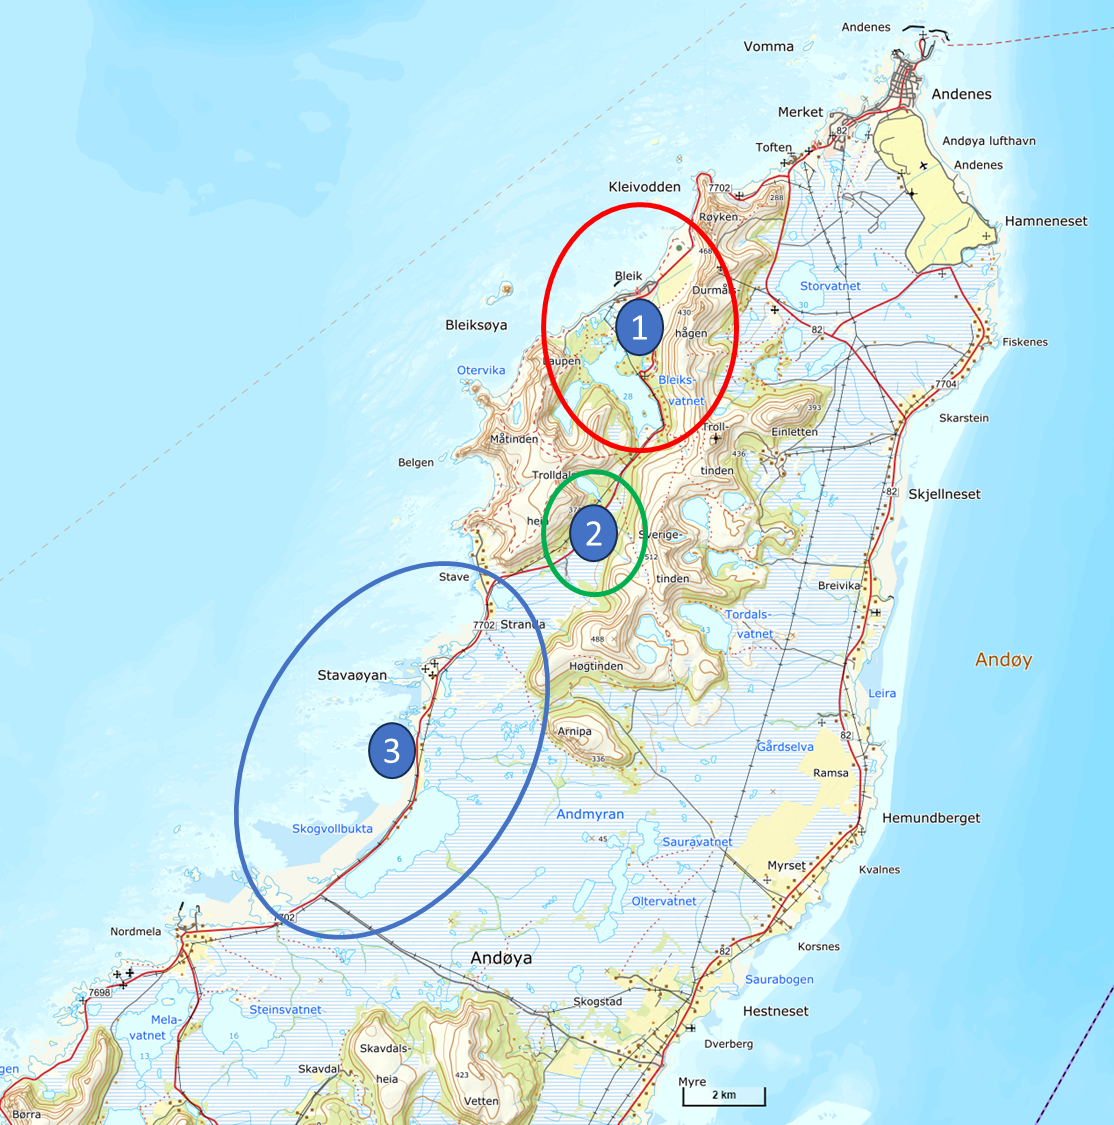
\includegraphics[width = 0.5\textwidth]{test_sites}
\end{center}

For each of the sites there will be there may be several points of different types. Houses, transmitters, parkinglots, motorcade routes and drone areas. There is a corresponding geojson file that can be opened in geojson.io or in any decent GIS application like Qgis. The geojson file contains points, line and polygons.

\section*{Site 1 - Bleik (69.275696N, 15.968345E)}
The Bleik community house is the main location during Jammertest. This is the head quarter of the Jammertest organization and the big mess hall where the morning and evening briefing will be held and this is also where lunch for participants at site 1 will be served. The red dot marks the community house.\\

\begin{center}
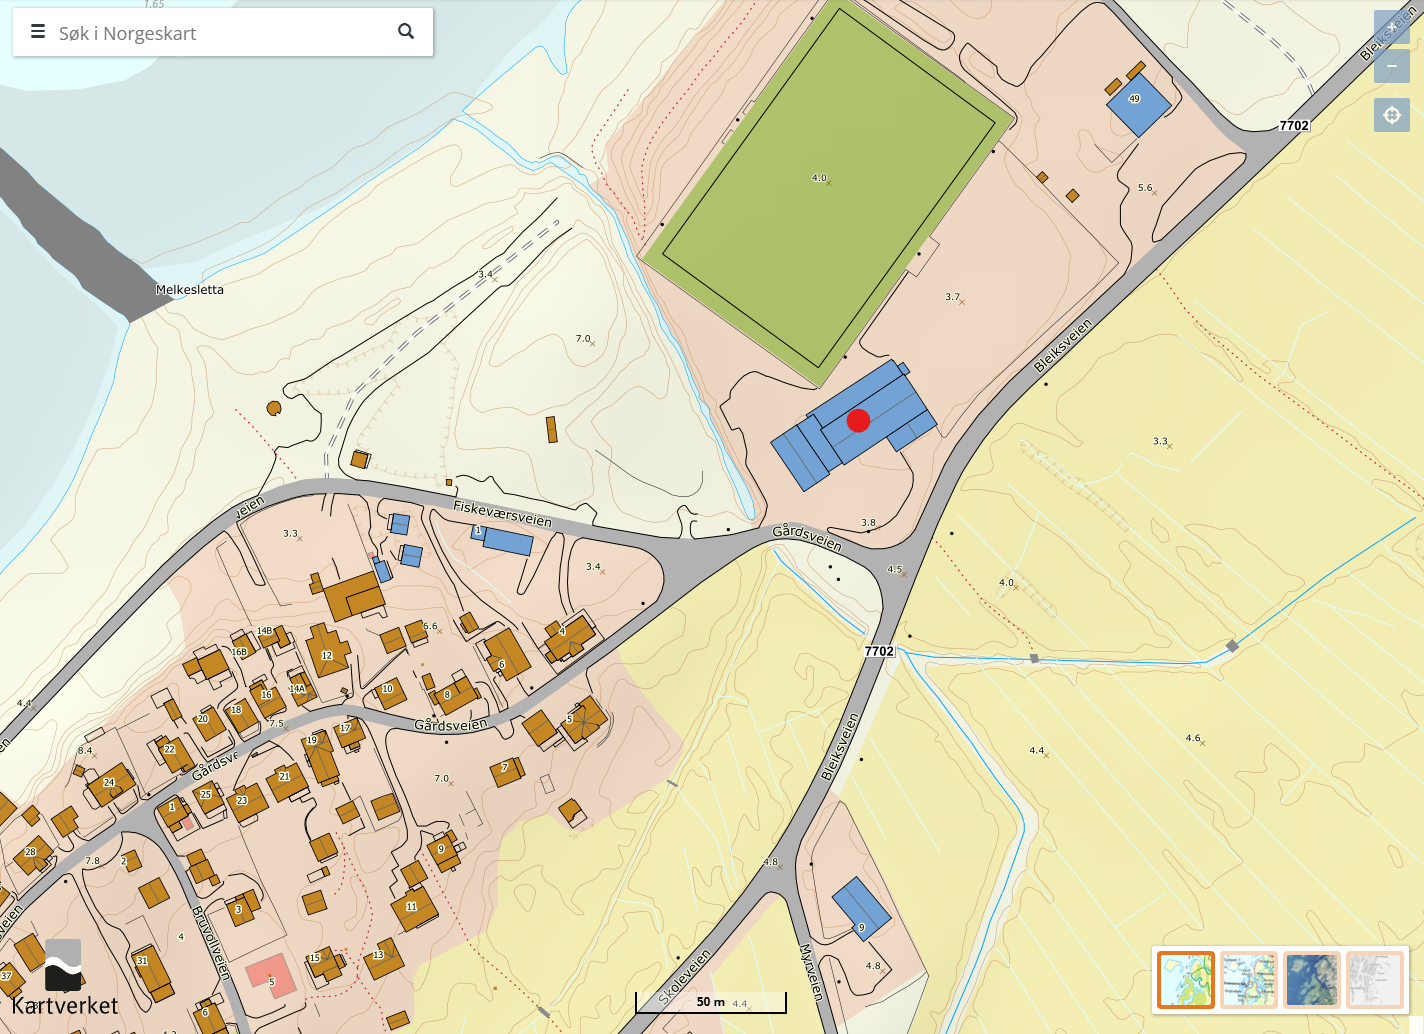
\includegraphics[width = 0.7\textwidth]{bleik}\\
\end{center}
At site 1 equipment can be placed on the lawn to the north of the community house, in and on vehicles stationed outside the community house. Vehicles are also free to use the public roads in the area to move in and out of the jammed area.



\section{Site 2 - Grunnvatnet (69.222476N, 15.933461E)}
Grunnvatnet is well suited for testing of smaller and lower power jammers. The area consist of a gravel road and parkinglot where vehicles can be stationed. The area is also well suited for flying drones while beeing jammed. At this site there is typically a mix of organized sessions and bookable time where test can be more tailored to the test group. Jammers and or equipment can be placed in the terrain surrounding in parkinglot and gravel roads. Red dot marks the Grunnvatnet parkinglot.\\

\begin{center}
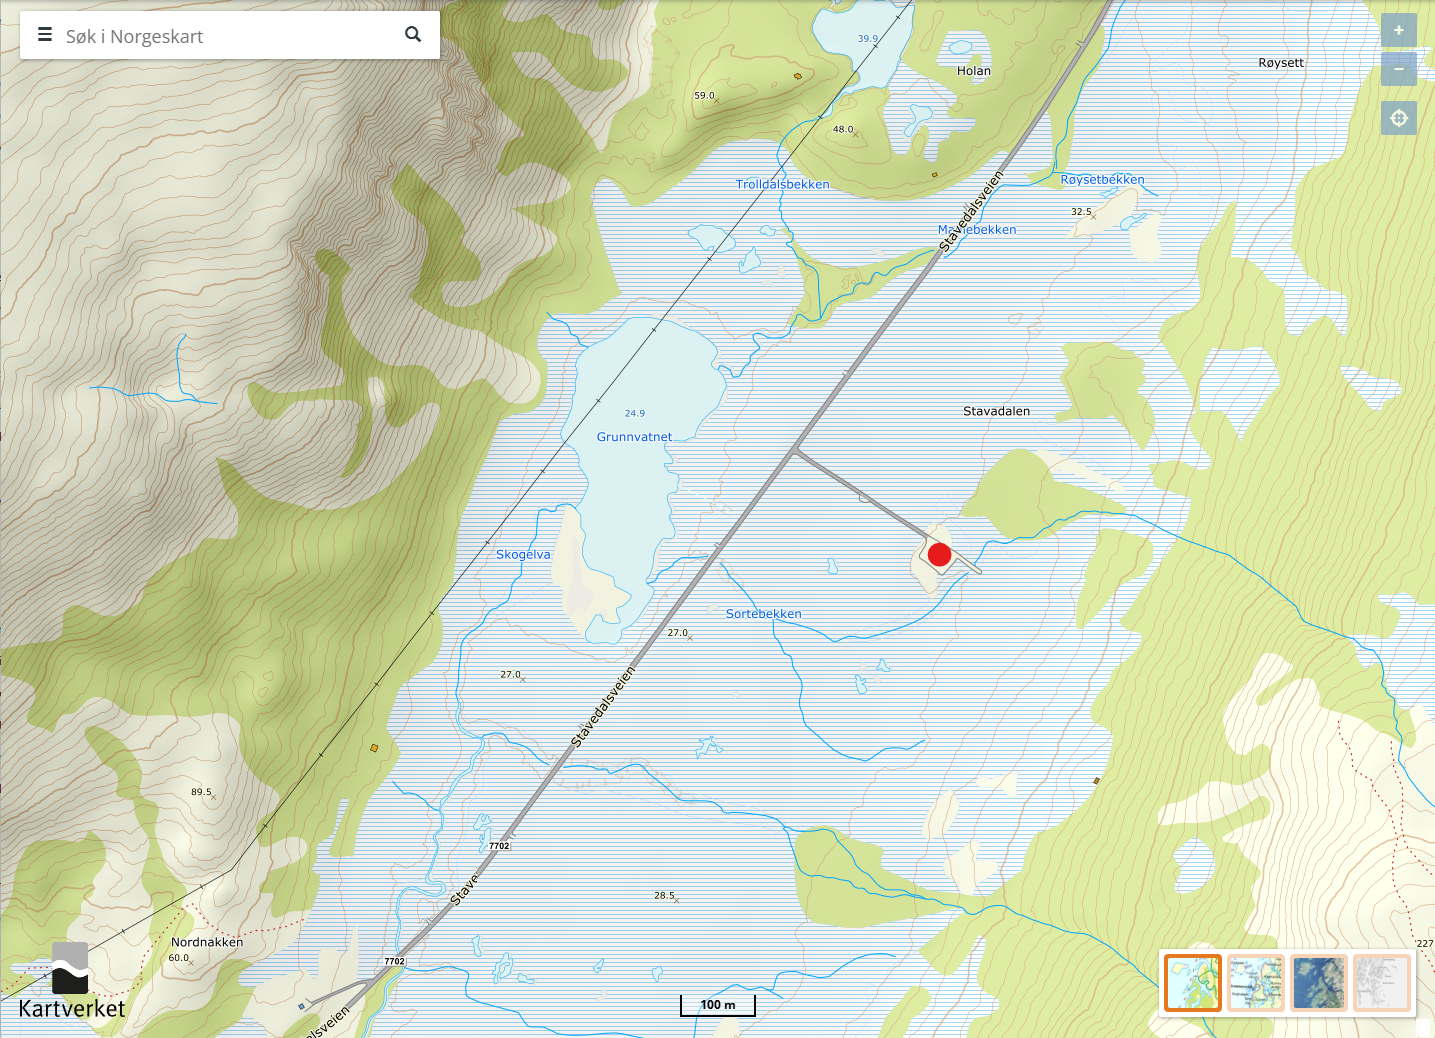
\includegraphics[width = 0.7\textwidth]{grunnvatnet.png}\\
\end{center}

For multi jammer tests a pattern like the one showed above will be used. The location of the spesific points are found in the geojson file.\\

\begin{center}
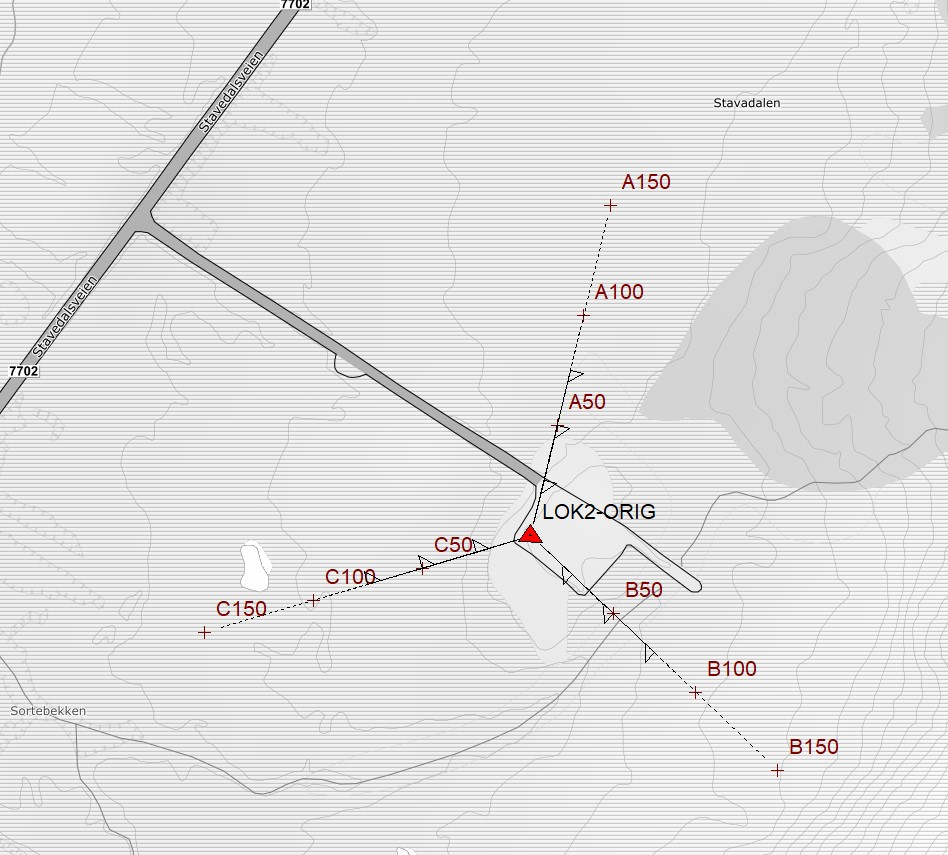
\includegraphics[width = 0.7\textwidth]{site_2_pattern.jpeg}\\
\end{center}

\section{Site 3 - Stave (69.212458N, 15.858584E)}
The Stave test site also has its own community house and is an area dedicated for motorcades. At this site there will be organized tests and bookable slots for more custom tests. Jammers can be placed both in vehicles and along the road depending on the tests. At this site only low powered jammers and spoofers are used. \\


\begin{center}
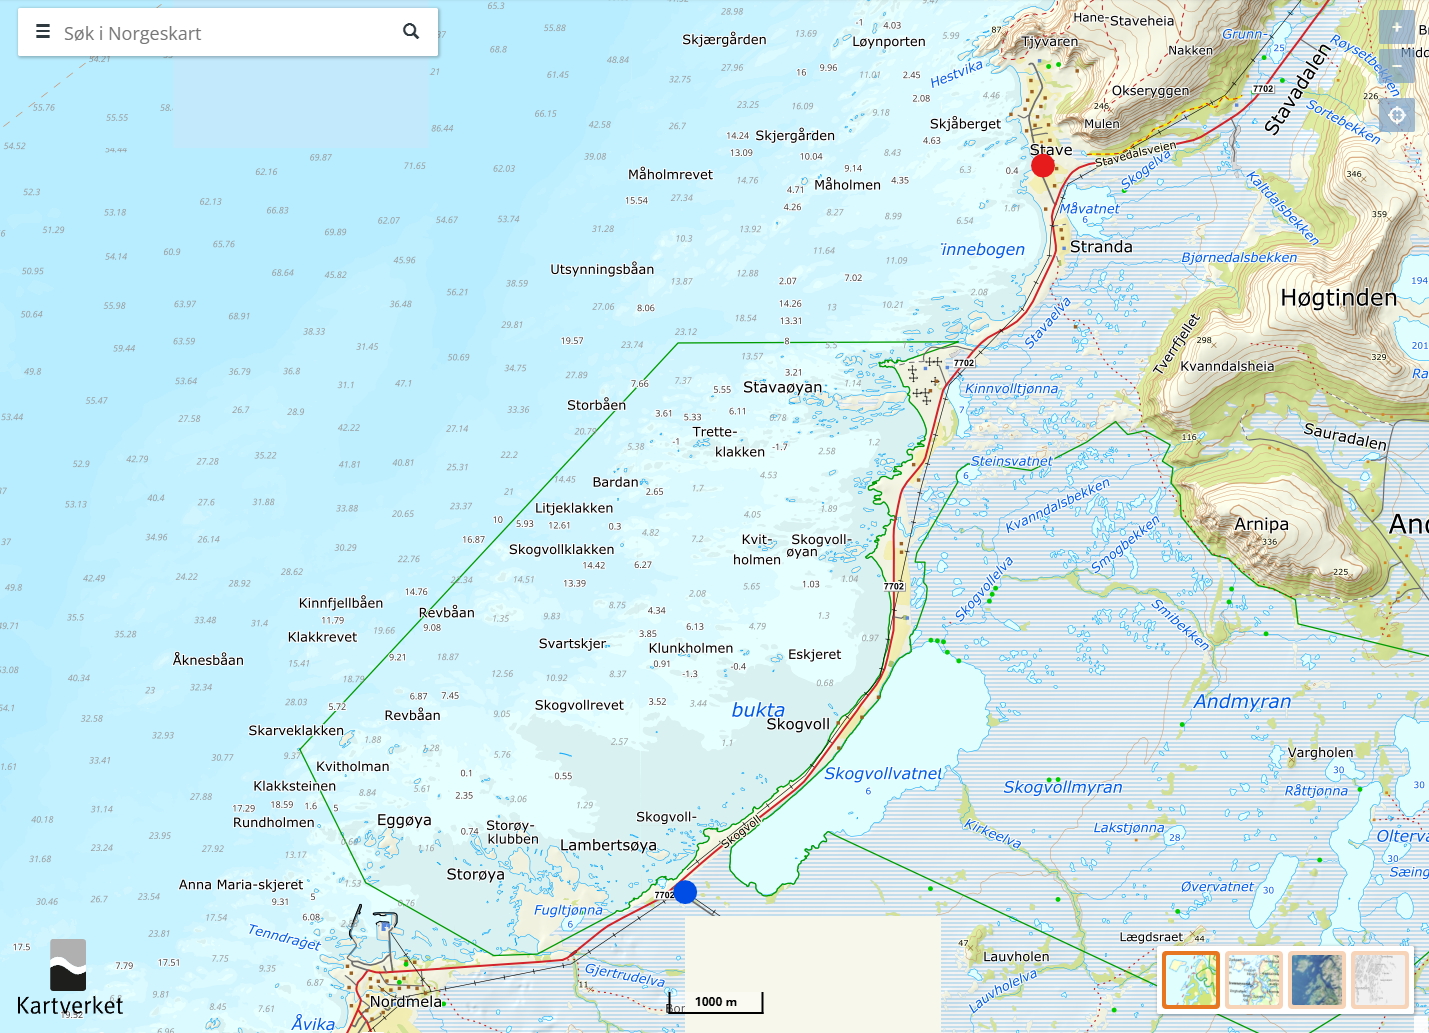
\includegraphics[width = \textwidth]{stave.png}\\ 
\end{center}

The red dot marks the Stave community house. The blue dot marks the southerns most point where jammers can be used. This means that typical motorcades will run somewhere between the red and blue dot. The geojson file contains the routes used by motorcades.